\documentclass[letterpaper,10pt,titlepage]{article}

\usepackage{graphicx}                                        
\usepackage{amssymb}                                         
\usepackage{amsmath}                                         
\usepackage{amsthm}                                          

\usepackage{alltt}                                           
\usepackage{float}
\usepackage{color}
\usepackage{url}

\usepackage{balance}
\usepackage[TABBOTCAP, tight]{subfigure}
\usepackage{enumitem}
\usepackage{pstricks, pst-node}

\usepackage{geometry}
\geometry{textheight=9in, textwidth=6.5in}

\newcommand{\cred}[1]{{\color{red}#1}}
\newcommand{\cblue}[1]{{\color{blue}#1}}

\usepackage{hyperref}
\usepackage{geometry}

\usepackage{listings}


\def\name{Sean Penney and Paul Atkinson}

%% The following metadata will show up in the PDF properties
\hypersetup{
  colorlinks = true,
  urlcolor = black,
  pdfauthor = {\name},
  pdfkeywords = {cs472 ``computer architecture'' clements ``chapter 3''},
  pdftitle = {CS 472: Homework 4},
  pdfsubject = {CS 472: Homework 4},
  pdfpagemode = UseNone
}

\begin{document}
\hfill \name

\hfill \today

\hfill CS 472 HW 4

\begin{enumerate}

\item[$(3.8)$]

  The benefit of a general purpose register is that it can be used for many different actions, and can switch up what it is doing mid program.
  However, being general makes it so there is memory wasted indicating what it would be doing. A single purpose register can then use a lot more
  of its available memory.

\item[$(3.9)$] 

  A misaligned operand is one that is not aligned on the word boundaries of the system.
  
  Misaligned operands are an issue, because 2 memory location may need to be read to get an operand if it is not properly aligned.
  Reading 2 memory locations to get one operand is inefficient

\item[$(3.24)$]

  P = Pointer adjust, Pre or post increment
  
  U = Pointer direction, Up or Down

  B = Word Access

  W = Pointer update, Write back

  L = Data direction, Load or Store

\item[$(3.26)$] 

  The register r6 shifted to the left by the value in r2.  The result is added to r5.  This becomes the effective address for data that is loaded into r0.
  
\item[$(3.30)$]

  When a number is copied into a location where there are more bits for that number, it uses the sign-extension. Sign-extension takes the 
  sign bit and extends it out for however many extra bits there are. What this means is, if you have a number 10 for instance, which is 00001010 
  in binary and you store that 8 bit number into a 16 bit number, it then looks like 0000000000001010.

\item[$(3.33)$] 

  Block move instructions are useful since a block of registers can be copied to or from memory with a single instruction.
  Block moves are easy to understand, however, there are many options that determine how the move takes place which can complicate things.

\item[$(3.34)$]

  This instruction copies the registers r0 to r2 and r4 into sequential memory locations using r13 as a pointer with auto indexing. 
  Since it has the IA suffix, the register r13 is incremented after each transfer.


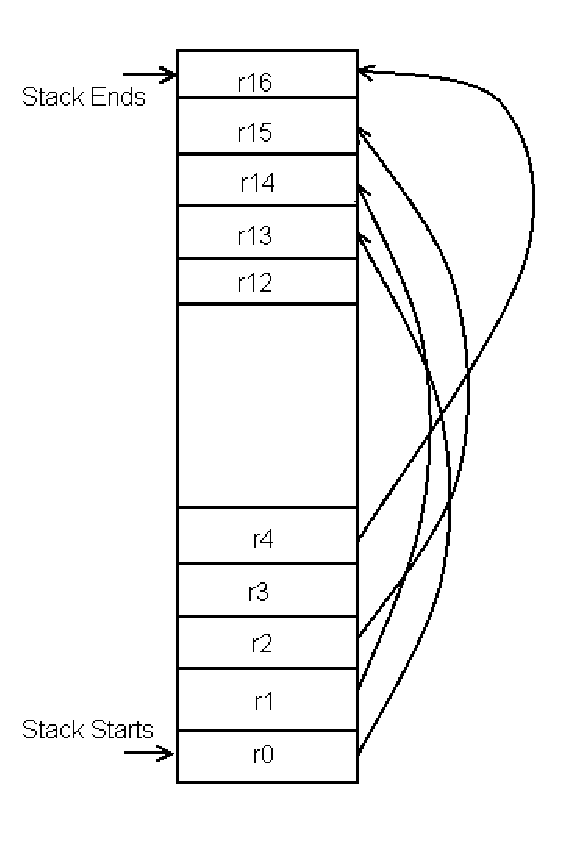
\includegraphics[scale=.5]{stack.eps}


\item[$(3.36)$] 

  Let r0 be the register we are multiplying by a given value.
  
  a. (r0 << 5) + r0
  
  b. (ro << 10) + r0
  
  c. (r0 << 12) - r0 

\item[$(3.44)$]

  It makes r0 a positive version of itself.

\item[$(3.48)$]

  A pseudo-operation do not directly translate to a machine instruction.  They are resolved by the assembler during assembly.
  Pseudo operations generally give information such as data alignment or symbol definitions.
  
\item[$(3.54)$]

\begin{lstlisting}
	MOV r1, #0 		; This sets r1 to the value of 0
loop	MOVS r0, r0, LSL #1 	; Increments r0 by 1
	ADDCC r1, r1, #1	; Increments r1 by 1
	BCC loop		; It loops if the carry bit is cleared
\end{lstlisting}

  It turns r1 into the max registery size - r0.

\item[$(3.60)$]

\begin{lstlisting}
AREA vector, CODE, READONLY
		ENTRY

VECTOR	MOV r0, #8			; loop 8 times
	ADR r1, VECA
	ADR r2, VECB
	ADR r3, VECC
LOOP	LDR r4, [r1], #4	; get element from VECA, post increment address
	LDR r5, [r2], #4	; get element from VECB, post increment address
	ADD r6, r4, r5		; add elements from VECA and VECB
	LSR r6, r6, #1		; shift result to right (divide by 2)
	STR r6, [r3], #4	; store result in VECC and post increment address
	SUBS r0, r0, #1		; decrement loop counter and set status flag
	BNE LOOP			; continue untsil loop counter is 0
	MOV pc, lr			; Return from subroutine
		
AREA vector, DATA, READWRITE
VECA	DCD 1,2,3,4,5,6,7,8 ; 8 element vector
VECB	DCD 1,2,3,4,5,6,7,8 ; 8 element vector
VECC	DCD 0,0,0,0,0,0,0,0 ; 8 element vector
\end{lstlisting}
  
\item[$(3.61)$]

  The register r15 could not be used in conjunction with most data processing instructions because the program counter has certain values that would be valid.
  Instructions are four bytes long, so r15 can only be changed in increments of 4.  Also, the PC has to point to an actual instruction in the program.
  
\end{enumerate}



\end{document}
